\documentclass[a4paper, notitlepage]{article}
%\usepackage[cm]{fullpage}
\usepackage[pdftex]{graphicx}
\usepackage{float}

\begin{document}

\title{Installation and User Guide} 
\date{\today}
\maketitle



\section{Requirements}

\begin{itemize}
	\item Internet connection
	\item The following tools must be installed (lower versions may work, but not recommended)
	\begin{itemize}
		\item \textit{Java SDK} ($>=$ 7)
		\item \textit{Git} - to get the code - http://git-scm.com/downloads
		\item \textit{Maven} ($>=$ 3) - for building - http://maven.apache.org/download.html
		\item \textit{Apache Tomcat} ($>=$ 8) - for deploying the web interface - http://tomcat.apache.org/
	\end{itemize}
\end{itemize}

\section{Get the code}
Using Git clone the repository hosted at GitHub using the following command:

\textit{git clone https://github.com/btodorov88/springbank.git}

\section{Build the project}

In order to build the project the following steps have to be executed using \textit{Command Prompt} or alternative:
\begin{enumerate}
	\item Navigate to the SpringBankWeb folder in the cloned repository
	\item Execute the \textit{mvn clean package} command
\end{enumerate}

\section{Deploy}
The build procedure creates deployable \textit{war} file. It can be found at \textit{SpringBankWeb\textbackslash target\textbackslash springbank-1.0.0-BUILD-SNAPSHOT}. In order to deploy the file, one has to copy it to the \textit{webapps} folder of the Tomcat web server (for easier access the file should be renamed to \textit{springbank.war}). Once deployed the web client can be accessed at \textit{localhost:8080\textbackslash springbank} (default Tomcat configuration).


\section{Explore the application}

When the application is started it redirects to a login page for authentication (Figure \ref{login}). The test data sets up user \textit{btodorov} with password \textit{123} that can be used to login. Once successfully authenticated the user is redirected to the main page which presents all accounts (left table) and transactions (right table) associated with the authenticated user (Figure \ref{main}). 

\bigskip
\begin{figure}[H]
  \centering
    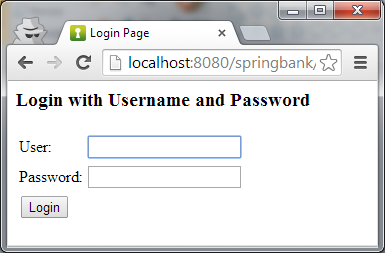
\includegraphics[width=0.6\textwidth]{login_Screen.png}
    \caption{Initial login view}
    \label{login}
\end{figure}
\bigskip

A new bank transaction can be made by clicking on the "Create transaction" button in the menu. Then the user is asked to fill in a form providing details about the transaction (Figure \ref{new}). When the form is submitted it is validated to make sure all necessary fields are populated and the "From account" has enough capital. In case of success the user is redirected to the main page where the newly created transaction can be seen.
 
\bigskip
\begin{figure}[H]
  \centering
    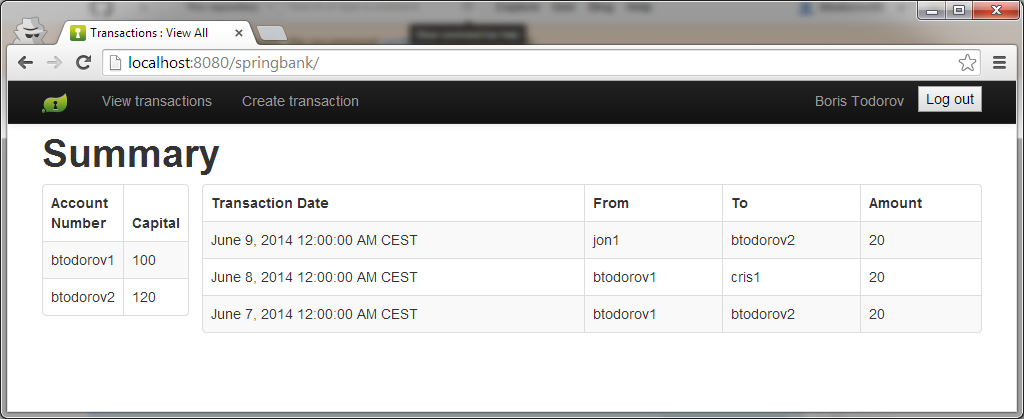
\includegraphics[width=0.9\textwidth]{main_Screen.png}
    \caption{The main view which summarizes the accounts and transactions associated with the authenticate user}
    \label{main}
\end{figure}
\bigskip

\begin{figure}[H]
  \centering
    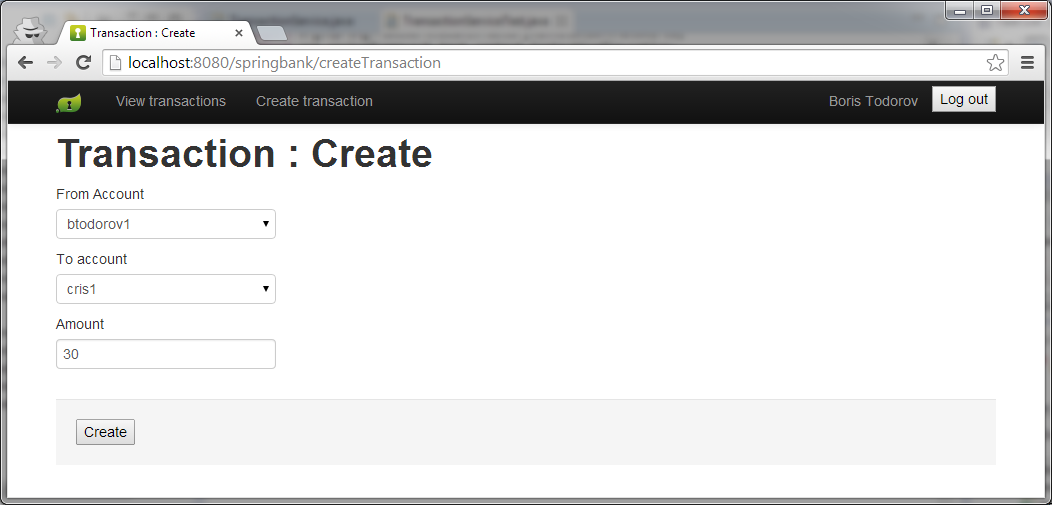
\includegraphics[width=0.8\textwidth]{new_Screen.png}
    \caption{The form that has to be filled in in order to create a new transaction}
    \label{new}
\end{figure}

\section{Take a look at the code}
The cloned project can be easily imported into Eclipse. In order to do that go to \textit{File\textbackslash Import \textbackslash Existing Projects into Workspace} and follow the instructions.

Next section briefly presents the internal organization of the system and identifies the high level components that it is built of. 

\subsection{Architecture}

The architecture of the application is illustrated in Figure \ref{org}. It consists of the following components:
\bigskip

\begin{figure}[H]
  \centering
    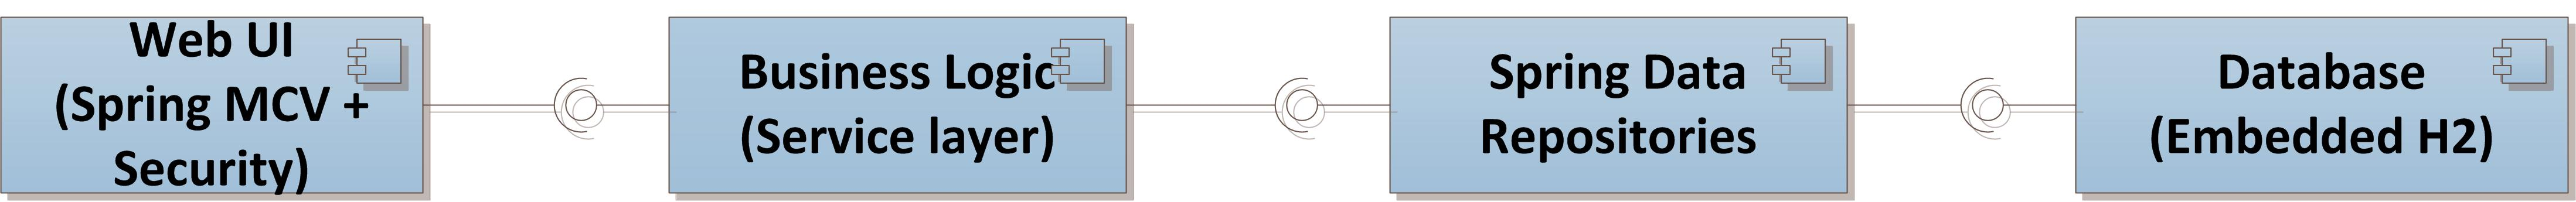
\includegraphics[width=1.3\textwidth]{high_level.jpg}
    \caption{Component diagram illustrating the functional organization of the system}
    \label{org}
\end{figure}


\bigskip
\begin{itemize}
	\item \textit{Database} - Responsible to store the accounts and transactions data. In the current implementation we use embedded H2 database for simplicity but it is just a matter of configuration to switch to another SQL database. On startup the database is populated with some test data.
	
	\item \textit{Spring data repositories} - This component uses JPA2 and Hibernate to provide CRUD stile interaction with the database. The main application data objects (Person, Account, Transaction) are represented as JPA entities. 
	
	\item \textit{Business logic} - This component defines the Spring services which encapsulate the main business logic of the application.
	
	\item \textit{Web UI} - This component is responsible to provide the Web interface of the application. It uses Spring MVC in combination with Thymeleaf and Apache Tiles to render the views presented to the users. The application also uses Spring Security to manage the access to its functionality. It uses the user information from the database (Person) for authentication.
\end{itemize}


\end{document}